\documentclass[11pt,german,table,dvipsnames]{beamer}
\usetheme{ubslides}

\usepackage[labelformat=empty,font=tiny]{caption}
\usepackage{graphicx}
\usepackage{booktabs}
\usepackage{multicol}
\usepackage{fancyvrb}



%\setbeameroption{show notes on second screen=right}

%%% set up literature
\setbeamertemplate{bibliography item}{\insertbiblabel}
\usepackage[%
  backend=bibtex      % biber or bibtex
%,style=authoryear    % Alphabeticalsch
 ,style=numeric-comp  % numerical-compressed
 ,sorting=none        % no sorting
 ,sortcites=true      % some other example options ...
 ,block=none
 ,indexing=false
 ,citereset=none
 ,isbn=true
 ,url=true
 ,doi=true            % prints doi
 ,natbib=true         % if you need natbib functions
]{biblatex}


% set up stuff for the title page and slides footer
\title{Fail2ban Evaluierung}
\author[Paul Raatschen]{Paul Raatschen}
\date{1. Dezember 2022}
\institute[Uni Potsdam]{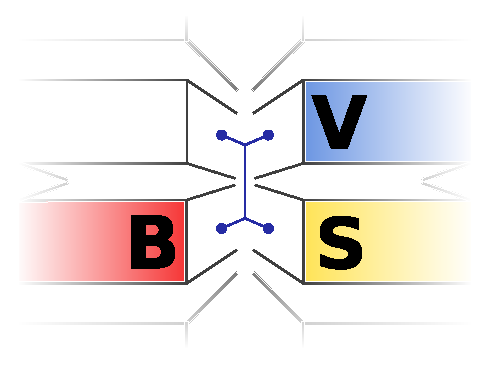
\includegraphics[width=1.5cm]{images/bsvs-logo.eps}}%\\Universtität Potsdam\\ Institut für Informatik und Computational Science\\ Professur Betriebssysteme und Verteilte Systeme}

\setbeamertemplate{caption}{\insertcaption}

\usepackage{hyperref}

\begin{document}

\begin{frame}[plain]
    \titlepage
\end{frame}

\begin{frame}
\frametitle{Übersicht}

\begin{itemize}
    \item Grundlagen  
        \begin{itemize}
        \item Fail2ban 
        \item eBPF
    \end{itemize}
    \item Messungen
    \begin{itemize}
        \item Raw UDP Traffic
        \item DNS Traffic
        \item HTTP Traffic
    \end{itemize}
    
\end{itemize}

\end{frame}

\section{Grundlagen}

\subsection{Fail2ban}

\begin{frame}{Fail2ban}
    \begin{itemize}
        \item Open Source Intrusion Prevention System.
        \item Blockiert ungewollten Datenverkehr auf Basis von Anwendungs-Logdateien.
        \item Fail2ban erlaubt die Konfiguration von ``Jails''.
        \item Ein Jail besteht aus Filter, Action sowie Paramtern. 
    \end{itemize}
\end{frame}

\begin{frame}[fragile]{Jail Parameter und Filter}

\begin{Verbatim}[fontsize=\small]
# Jail Definition
[udp-testsvr]
port    = 8080
logpath = /mnt/scratch/PR/udpsvr.log
enabled = true
filter  = udp-testsvr
findtime = 10
bantime = 180
action = xdp
maxretry = 0

# Filter
[Definition]
failregex = Address = <HOST>, Port = \d{1,5}, Payload = 2\d{2}
datepattern =  %%Y-%%b-%%d %%H:%%M:%%S
\end{Verbatim}
\end{frame}

\subsection{eBPF}

\begin{frame}{eBPF}

\begin{itemize}
    \item Extended Berkley Packet Filter. Interface im Linux Kernel.
    \item Erlaubt ereignisbasierte Ausführung von Benutzerprogrammen im Kernel, u.a. für Paketfilterung.
    \item Kann für Fail2ban an Stelle von Iptables verwendet werden. 
\end{itemize}
    
\end{frame}

\begin{frame}{Fail2ban + eBPF}

\begin{figure}
    \centering
    \includegraphics[width=\textwidth]{images/architektur_ebpfoverall2.png}
    \caption{Quelle: Florian Mikolajczak : ``Implementation and Evaluation of an Intrusion
Prevention System Leveraging eBPF \\ on the
Basis of Fail2Ban'', Master Thesis, 2022 }
\end{figure}

    
\end{frame}

\section{Messungen}

\begin{frame}{Testumgebung}

\begin{table}[b!]
	 \centering
	\begin{tabular}{ll}
	\toprule
	\multicolumn{2}{l}{\textbf{Hardware}}                                        \\ \midrule
	\textbf{CPU}        & 16 x Intel Xeon Silver 4314 CPU @ 2.4GHz \\
	\textbf{NIC}        &  Mellanox ConnectX-5 100Gb/s Ethernet                     \\
	\textbf{RAM}        & 131.4GB                                                       \\ \bottomrule 
	\multicolumn{2}{l}{\textbf{Software}}                                        \\ \midrule
	\textbf{OS}         & Debian 10                                                  \\
	\textbf{Kernel}          & 5.15.7                                                     \\
	\textbf{NIC Driver}  & mlx5\_core 5.5-1.0.3                                      \\
	\textbf{BIND}       & 9.11.5                                    \\
    \textbf{Nginx} & 1.14.2 \\
	\textbf{Fail2Ban}       & 0.11.2                                   \\
	\textbf{TRex}            & 2.99                                        \\ \bottomrule
	\end{tabular}
	\end{table}

    
\end{frame}

\subsection{Raw UDP}
    
\begin{frame}{Raw UDP Traffic}
    \begin{itemize}
        \item Minimaler (single-threaded) Server, der UDP Anfragen beantwortet.
        \item Problem: Schwache Performance, schafft nur $\sim$100k Anfragen pro Sekunde.
        \item Messung: Client (Trex auf bsnode2) sendet UDP Pakete mit 1 Byte Payload an Server (bsnode1). 
        \item Mischung aus validem und invalidem Traffic.
        \item Variablen: Packets per second (PPS) und Anzahl der Clients.
    \end{itemize}
\end{frame}

\begin{frame}{}
    \begin{figure}
        \centering
        \includegraphics[width=1.1\textwidth]{images/udp_10_50_50.png}
    \end{figure}
\end{frame}

\begin{frame}{}
    \begin{figure}
        \centering
        \includegraphics[width=1.1\textwidth]{images/udp_10_50_254.png}
    \end{figure}
\end{frame}

\subsection{DNS}

\begin{frame}{DNS Traffic}
    \begin{itemize}
        \item Client (Trex auf bsnode2) schickt DNS Requests an BIND Server (bsnode1).
        \item Variablen: Packets per Second (PPS) und Anzahl der Clients.
    \end{itemize}
\end{frame}

\begin{frame}{}

\begin{figure}
    \centering
    \includegraphics[width=1.1\textwidth]{images/dns_50_1000_50.png}
\end{figure}
    
\end{frame}
\begin{frame}

\begin{figure}
    \centering
    \includegraphics[width=1.1\textwidth]{images/dns_50_5000_50.png}
\end{figure}
    
\end{frame}

\begin{frame}

\begin{figure}
    \centering
    \includegraphics[width=1.1\textwidth]{images/dns_50_1000_254.png}
\end{figure}
    
\end{frame}

\begin{frame}

\begin{figure}
    \centering
    \includegraphics[width=1.1\textwidth]{images/dns_50_5000_254.png}
\end{figure}
    
\end{frame}

\subsection{HTTP}

\begin{frame}{HTTP Traffic}
    \begin{itemize}
        \item Client (Trex auf bsnode2) schickt HTTP GET Request an Nginx Server (bsnode1).
        \item 8 TCP Pakete pro Verbindung (inklusive Handshake).
        \item Variablen: Connections per second (CPS).
        \item Problem: Trex liefert nicht die spezifizierte Anzahl an CPS.
    \end{itemize}
    
\end{frame}

\begin{frame}{}
    \begin{figure}
    \centering
    \includegraphics[width=1.1\textwidth]{images/http_50_100.png}
\end{figure}
\end{frame}

\begin{frame}{}
    \begin{figure}
    \centering
    \includegraphics[width=1.1\textwidth]{images/http_50_1000.png}
\end{figure}
\end{frame}

\pagenumbering{arabic}

\end{document}
